  %%%%%%%%%%%%%%%%%%%%%%%%%%%%%%%%%%%%%%%%%

% Short Sectioned Assignment
% LaTeX Template
% Version 1.0 (5/5/12)
%
% This template has been downloaded from:
% http://www.LaTeXTemplates.com
%
% Original author:
% Frits Wenneker (http://www.howtotex.com)
%
% License:
% CC BY-NC-SA 3.0 (http://creativecommons.org/licenses/by-nc-sa/3.0/)
%
%%%%%%%%%%%%%%%%%%%%%%%%%%%%%%%%%%%%%%%%%

%----------------------------------------------------------------------------------------
%   PACKAGES AND OTHER DOCUMENT CONFIGURATIONS
%----------------------------------------------------------------------------------------

\documentclass[paper=a4, fontsize=11pt]{scrartcl} % A4 paper and 11pt font size

\usepackage[T1]{fontenc} % Use 8-bit encoding that has 256 glyphs
\usepackage{palatino} % Use the Adobe Utopia font for the document - comment this line to return to the LaTeX default
\usepackage[english]{babel} % English language/hyphenation
\usepackage{amsmath,amsfonts,amsthm} % Math packages
\usepackage{multicol,lastpage,fullpage,framed,fancybox,enumerate,tikz}
\usepackage{lipsum} % Used for inserting dummy 'Lorem ipsum' text into the template
\usepackage{mathrsfs}
\usepackage{graphicx}
\usepackage{mathtools}
\usepackage{url}

\usepackage{color}   %May be necessary if you want to color links
\usepackage{hyperref}
\hypersetup{
    colorlinks=true, %set true if you want colored links
    linktoc=all,     %set to all if you want both sections and subsections linked
    linkcolor=blue,  %choose some color if you want links to stand out
}



\AtBeginEnvironment{bmatrix}{\setlength{\arraycolsep}{1.5pt}}
%
%
%
%   A T T E N T I O N ! ! !
%
%   SET YOUR GRAPHICS FOLDER IN THE LINE BELOW
%
\graphicspath{ {.} }
\usepackage{sectsty} % Allows customizing section commands
\allsectionsfont{\centering \normalfont\scshape} % Make all sections centered, the default font and small caps

\usepackage{fancyhdr} % Custom headers and footers
\pagestyle{fancy plain} % Makes all pages in the document conform to the custom headers and footers
\fancyhead[L]{\textsc{CSEN 5830}}
\fancyhead[R]{\textsc{Homework #3}} % No page header - if you want one, create it in the same way as the footers below
\fancyfoot[L]{} % Empty left footer
\fancyfoot[C]{} % Empty center footer
\fancyfoot[C]{- \thepage -} % Page numbering for right footer
\renewcommand{\headrulewidth}{0.5pt} % Remove header underlines
\renewcommand{\footrulewidth}{0pt} % Remove footer underlines
\setlength{\headheight}{13.6pt} % Customize the height of the header

\fancypagestyle{noheader}{    %create style that allows to skip header manually on pages with new section
    \fancyhead{}
    \renewcommand{\headrulewidth}{0pt}
}

\numberwithin{equation}{section} % Number equations within sections (i.e. 1.1, 1.2, 2.1, 2.2 instead of 1, 2, 3, 4)
\numberwithin{figure}{section} % Number figures within sections (i.e. 1.1, 1.2, 2.1, 2.2 instead of 1, 2, 3, 4)
\numberwithin{table}{section} % Number tables within sections (i.e. 1.1, 1.2, 2.1, 2.2 instead of 1, 2, 3, 4)

\setlength\parindent{0pt} % Removes all indentation from paragraphs - comment this line for an assignment with lots of text

%----------------------------------------------------------------------------------------
%   TITLE SECTION
%----------------------------------------------------------------------------------------

\newcommand{\horrule}[1]{\rule{\linewidth}{#1}} % Create horizontal rule command with 1 argument of height

\title{
\normalfont \LARGE
\textsc{University of Colorado at Boulder} \\ [25pt] % Your university, school and/or department name(s)
\textsc{ASEN 5044 - Statistical State Estimation for Dynamical Systems} \\ [20pt]
\textsc{Fall 2024} \\ [20pt]
\textsc{Professor: Dr. Nisar Ahmed} \\ [12pt]
\horrule{1pt} \\[0.4cm] % Thin top horizontal rule
\huge Project Report 1 \\ % The assignment title
\huge (Cooperative Air-Ground Robot Localization) \\ 
\horrule{1pt} \\[0.6cm] % Thick bottom horizontal rule
}

\author{
  \textsc{ Team Members:} \\ [4 mm]
  \textsc{ Nicholas Martinez}\\[2mm]
  \textsc{ Whit Whittall } \\[2mm]
  \textsc{ Michael Bernabei}\\[2mm]
}

\date{\normalsize\today} % Today's date or a custom date

\begin{document}

\maketitle % Print the title
\thispagestyle{empty} %make title page header empty
\newpage

\tableofcontents

\listoffigures


\newpage

%----------------------------------------------------------------------------------------
%   PROBLEM SECTION
%----------------------------------------------------------------------------------------
%

\section{Progress Reports}
\subsection{Progress Report For Part I}
\begin{framed}

\textbf{Team Member Contributions} \\
Nicholas Martinez:
\begin{enumerate}
    \item Nonlinear System Modeling with ODE45
\end{enumerate}
Whit Whittall:
\begin{enumerate}
    \item Linearized DT LTV System Modeling
\end{enumerate}
Micheal Bernabei
\begin{enumerate}
    \item Computation of CT Jacobian Matrices
\end{enumerate}

Our group is nearly complete with Part I Deterministic System Analysis. At this time, we’ve computed the CT Jacobian matrices. This yielded a time varying system, so we have skipped observability and stability analysis. We performed a full nonlinear simulation of the system dynamics. We simulated the linearized DT dynamics and validated these results against the nonlinear simulation and the posted “solution sketches” on canvas. Our results match the posted results on canvas. The only thing we have not done at this stage is simulated the measurement models.

\end{framed}

\newpage


%----------------------------------------------------------------------------------------
%   PROBLEM SECTION
%----------------------------------------------------------------------------------------
%
\subsection{Progress Report For Part II}
\begin{framed}

\textbf{Team Member Contributions} \\
Nicholas Martinez:
\begin{enumerate}
    \item tbd
\end{enumerate}
Whit Whittall:
\begin{enumerate}
    \item tbd
\end{enumerate}
Micheal Bernabei
\begin{enumerate}
    \item tbd
\end{enumerate}

 tbd

\end{framed}


\newpage


\section{Part I. of Cooperative Air-Ground Robot Localization}
\begin{framed}
\subsection{Part I} \\

We are given the Equation Of Motion (EOM) for the Unmanned Ground Vehicle (UGV).  The EOM is,

\begin{align*}
    \dot{\xi_g} &= v_g \cos{\theta_g} + \Tilde{w}_{x,g} \\
    \dot{\eta_g} &= v_g \sin{\theta_g} + \Tilde{w}_{y,g} \\
    \dot{\theta_g} &= \frac{v_g}{L}\tan{\phi_g}  + \Tilde{w}_{\omega,g} \\
\end{align*}

and for the Unmanned Aerial Vehicle (UAV) we have the following EOM,

\begin{align*}
    \dot{\xi_a} &= v_a \cos{\theta_a} + \Tilde{w}_{x,a} \\
    \dot{\eta_a} &= v_a \sin{\theta_a} + \Tilde{w}_{y,a} \\
    \dot{\theta_a} &= \omega_a  + \Tilde{w}_{\omega,a} \\
\end{align*}

where $\Tilde{w}_a = [ \Tilde{w}_{x,a},  \Tilde{w}_{y,a},  \Tilde{w}_{\omega,a}]^T$ and $\Tilde{w}_g = [ \Tilde{w}_{x,g},  \Tilde{w}_{y,g},  \Tilde{w}_{\omega,g}]^T$ are the process noise for the UAV And UGV respectively.  We are also given the following sensing model,

\begin{align*}
y(t) &=  
\begin{bmatrix} \arctan{(\frac{\eta_a - \eta_g}{\xi_a - \xi_g}}) - \theta_g   \\ 
                \sqrt{  (\xi_g - \xi_a)^2 + (\eta_g - \eta_a)^2}  \\
                \arctan{(\frac{\eta_g - \eta_a}{\xi_g - \xi_a})} - \theta_a \\
                \xi_a \\
                \eta_a
\end{bmatrix}  + \Tilde{\bold{v}}(t) \\
\end{align*}

where $\Tilde{\bold{v}}(t) \in \mathbb{R}^5$ is the sensor error vector.  Finally, we are given the combined states, control inputs, and disturbance inputs as,

\begin{align*}
    \bold{x}(t) &= [ \xi_g \ \ \ \eta_g \ \ \ \theta_g \ \ \ \xi_a \ \ \ \eta_a \ \ \ \theta_a ] ^T ,\\
    \bold{u}(t) &= [ \bold{u}_g \ \ \bold{u}_a ]^T ,\\
    \bold{\Tilde{w}}(t) &= [\bold{\Tilde{w}_g \ \ \bold{\Tilde{w}}_a}]^T \\
\end{align*}

The state is $x = [\xi_g \ \  \eta_g \ \  \theta_g \ \  \xi_a \ \  \eta_a \ \ \theta_a ]^T = [ x_1 \ \ x_2 \  x_3 \ \ x_4 \ \ x_5 \ \ x_6 ]^T$ and our inputs $u = [ \bold{u}_g \ \ \bold{u}_a ]^T = [v_g \ \ \phi_g \ \ v_a \ \ \phi_a]^T = [u_1 \ \ u_2 \ \ u_3 \ \ u_4 ]^T$.  We then have the following after substituting in our state and input variables,

\begin{align*}
    \dot{x} &= \begin{bmatrix}
           \dot{\xi}_g \\
           \dot{\eta}_g \\
           \dot{\theta}_g \\
           \dot{\xi}_a \\
           \dot{\eta}_a \\
           \dot{\theta}_a
         \end{bmatrix} 
         =  \begin{bmatrix}
           \dot{x}_1 \\
           \dot{x}_2 \\
           \dot{x}_3 \\
           \dot{x}_4 \\
           \dot{x}_5 \\
           \dot{x}_6
         \end{bmatrix} 
         = \begin{bmatrix}
           \mathcal{F}_1(x,u) \\
           \mathcal{F}_2(x,u) \\
           \mathcal{F}_3(x,u) \\
           \mathcal{F}_4(x,u) \\
           \mathcal{F}_5(x,u) \\
           \mathcal{F}_6(x,u) \\
         \end{bmatrix}
         = \begin{bmatrix}
           u_1 \cos{x_3} \\
           u_1 \sin{x_3} \\
           \frac{u_1}{L} \tan{u_2} \\
           u_3 \cos{x_6} \\
           u_3 \sin{x_6} \\
           u_4 \\
         \end{bmatrix} 
\end{align*}


\begin{align*}
  y &= \begin{bmatrix} \arctan{(\frac{x_5 - x_2}{x_4 - x_1}}) - x_3   \\ 
                \sqrt{ (x_1 - x_4)^2 + (x_2 - x_5)^2}  \\
                \arctan{(\frac{x_2 - x_5}{x_1 - x_4})} - x_6 \\
                x_4 \\
                x_5
  \end{bmatrix} 
            = \begin{bmatrix}
           \mathcal{H}_1(x,u) \\
           \mathcal{H}_2(x,u) \\
           \mathcal{H}_3(x,u) \\
           \mathcal{H}_4(x,u) \\
           \mathcal{H}_5(x,u) \\
         \end{bmatrix}\\
\end{align*}
 
We now need to compute the partials of  $\mathcal{F}_{1\dots6}$ with respect to x,

\[ \begin{matrix*}[l]
\frac{\partial\mathcal{F}_1}{\partial x_1} = 0 &
\frac{\partial\mathcal{F}_2}{\partial x_1} = 0 & 
\frac{\partial\mathcal{F}_3}{\partial x_1} = 0 & 
\frac{\partial\mathcal{F}_4}{\partial x_1} = 0 & 
\frac{\partial\mathcal{F}_5}{\partial x_1} = 0 &  
\frac{\partial\mathcal{F}_6}{\partial x_1} = 0 & \\ \\
\frac{\partial\mathcal{F}_1}{\partial x_2} = 0 &
\frac{\partial\mathcal{F}_2}{\partial x_2} = 0 & 
\frac{\partial\mathcal{F}_3}{\partial x_2} = 0 & 
\frac{\partial\mathcal{F}_4}{\partial x_2} = 0 & 
\frac{\partial\mathcal{F}_5}{\partial x_2} = 0 &  
\frac{\partial\mathcal{F}_6}{\partial x_2} = 0 & \\ \\
\frac{\partial\mathcal{F}_1}{\partial x_3} = -u_1\sin{x_3} &
\frac{\partial\mathcal{F}_2}{\partial x_3} = u_1\cos{x_3} & 
\frac{\partial\mathcal{F}_3}{\partial x_3} = 0 & 
\frac{\partial\mathcal{F}_4}{\partial x_3} = 0 & 
\frac{\partial\mathcal{F}_5}{\partial x_3} = 0 &  
\frac{\partial\mathcal{F}_6}{\partial x_3} = 0 & \\ \\
\frac{\partial\mathcal{F}_1}{\partial x_4} = 0 &
\frac{\partial\mathcal{F}_2}{\partial x_4} = 0 & 
\frac{\partial\mathcal{F}_3}{\partial x_4} = 0 & 
\frac{\partial\mathcal{F}_4}{\partial x_4} = 0 & 
\frac{\partial\mathcal{F}_5}{\partial x_4} = 0 &  
\frac{\partial\mathcal{F}_6}{\partial x_4} = 0 & \\ \\
\frac{\partial\mathcal{F}_1}{\partial x_5} = 0 &
\frac{\partial\mathcal{F}_2}{\partial x_5} = 0 & 
\frac{\partial\mathcal{F}_3}{\partial x_5} = 0 & 
\frac{\partial\mathcal{F}_4}{\partial x_5} = 0 & 
\frac{\partial\mathcal{F}_5}{\partial x_5} = 0 &  
\frac{\partial\mathcal{F}_6}{\partial x_5} = 0 & \\ \\
\frac{\partial\mathcal{F}_1}{\partial x_6} = 0 &
\frac{\partial\mathcal{F}_2}{\partial x_6} = 0 & 
\frac{\partial\mathcal{F}_3}{\partial x_6} = 0 & 
\frac{\partial\mathcal{F}_4}{\partial x_6} = -u_3\sin{x_6} & 
\frac{\partial\mathcal{F}_5}{\partial x_6} = u_3\cos{x_6} &  
\frac{\partial\mathcal{F}_6}{\partial x_6} = 0 & \\ \\
\end{matrix*}\]

and with respect to u,

\[ \begin{matrix*}[l]
\frac{\partial\mathcal{F}_1}{\partial u_1} = \cos{x_3} &
\frac{\partial\mathcal{F}_2}{\partial u_1} = \sin{x_3} & 
\frac{\partial\mathcal{F}_3}{\partial u_1} = \frac{\tan{u_2}}{L} & 
\frac{\partial\mathcal{F}_4}{\partial u_1} = 0 & 
\frac{\partial\mathcal{F}_5}{\partial u_1} = 0 &  
\frac{\partial\mathcal{F}_6}{\partial u_1} = 0 & \\ \\
\frac{\partial\mathcal{F}_1}{\partial u_2} = 0 &
\frac{\partial\mathcal{F}_2}{\partial u_2} = 0 & 
\frac{\partial\mathcal{F}_3}{\partial u_2} = \frac{u_1}{L}\sec^2{u_2} & 
\frac{\partial\mathcal{F}_4}{\partial u_2} = 0 & 
\frac{\partial\mathcal{F}_5}{\partial u_2} = 0 &  
\frac{\partial\mathcal{F}_6}{\partial u_2} = 0 & \\ \\
\frac{\partial\mathcal{F}_1}{\partial u_3} = 0 &
\frac{\partial\mathcal{F}_2}{\partial u_3} = 0 & 
\frac{\partial\mathcal{F}_3}{\partial u_3} = 0 & 
\frac{\partial\mathcal{F}_4}{\partial u_3} = \cos{x_6} & 
\frac{\partial\mathcal{F}_5}{\partial u_3} = \sin{x_6} &  
\frac{\partial\mathcal{F}_6}{\partial u_3} = 0 & \\ \\
\frac{\partial\mathcal{F}_1}{\partial u_4} = 0 &
\frac{\partial\mathcal{F}_2}{\partial u_4} = 0 & 
\frac{\partial\mathcal{F}_3}{\partial u_4} = 0 & 
\frac{\partial\mathcal{F}_4}{\partial u_4} = 0 & 
\frac{\partial\mathcal{F}_5}{\partial u_4} = 0 &  
\frac{\partial\mathcal{F}_6}{\partial u_4} = 1 & \\ \\
\end{matrix*}\]

finally we compute $\mathcal{H}_{1 \dots 5}$ with respect to x.  In the following we show the two most complex partial derivative computations. The remaining partials were computed using similar techniques and therefore we omit them for brevity.  

Utilize the chain rule with $u=(\frac{x_5 - x_2}{x_4 - x_1})$, then, 
\\
\begin{align*}
    \frac{\partial{\mathcal{H}_1}}{\partial{x_1}} &= \frac{\partial{\mathcal{H}_1}}{\partial{u}} \times \frac{\partial{u}}{\partial{x_1}} \\
    &= \bigg( \frac{1}{(\frac{x_5 - x_2}{x_4 - x_1})^2 + 1} \bigg) \times \bigg(  \frac{0 \times (x_4-x_1) - (x_5-x_2)\times -1 }{(x_4 - x_1)^2}  \bigg) \\
    &= \bigg( \frac{1}{(\frac{x_5 - x_2}{x_4 - x_1})^2 + 1} \bigg) \times \bigg(  \frac{(x_5-x_2)}{(x_4 - x_1)^2}  \bigg) \\
    &= \bigg( \frac{1}{\frac{(x_5 - x_2)^2}{(x_4 - x_1)^2} + 1} \bigg) \times \bigg(  \frac{(x_5-x_2)}{(x_4 - x_1)^2}  \bigg) \\
    &= \bigg( \frac{1}{\frac{(x_5 - x_2)^2 + (x_4-x_1)^2}{(x_4 - x_1)^2}} \bigg) \times \bigg(  \frac{(x_5-x_2)}{(x_4 - x_1)^2}  \bigg) \\
    &= \bigg( \frac{(x_4 - x_1)^2}{(x_5 - x_2)^2 + (x_4-x_1)^2} \bigg) \times \bigg(  \frac{(x_5-x_2)}{(x_4 - x_1)^2}  \bigg) \\
    &= \frac{x_5-x_2}{(x_5 - x_2)^2 + (x_4-x_1)^2}
\end{align*}
\\
and we show the case when the partial we are computing is in the numerator,
\\
\begin{align*}
    \frac{\partial{\mathcal{H}_1}}{\partial{x_2}} &= \frac{\partial{\mathcal{H}_1}}{\partial{u}} \times \frac{\partial{u}}{\partial{x_2}} \\
    &= \bigg( \frac{1}{(\frac{x_5 - x_2}{x_4 - x_1})^2 + 1} \bigg) \times \bigg(  \frac{-1 \times (x_4-x_1) - (x_5-x_2)\times 0 }{(x_4 - x_1)^2}  \bigg) \\
    &= \bigg( \frac{1}{(\frac{x_5 - x_2}{x_4 - x_1})^2 + 1} \bigg) \times \bigg(  -\frac{(x_4-x_1)}{(x_4 - x_1)^2}  \bigg) \\
    &= \bigg( \frac{1}{\frac{(x_5 - x_2)^2}{(x_4 - x_1)^2} + 1} \bigg) \times \bigg(  -\frac{(x_4-x_1)}{(x_4 - x_1)^2}  \bigg) \\
    &= \bigg( \frac{1}{\frac{(x_5 - x_2)^2 + (x_4-x_1)^2}{(x_4 - x_1)^2}} \bigg) \times \bigg(  -\frac{(x_4-x_1)}{(x_4 - x_1)^2}  \bigg) \\
    &= \bigg( \frac{(x_4 - x_1)^2}{(x_5 - x_2)^2 + (x_4-x_1)^2} \bigg) \times \bigg(  -\frac{(x_4-x_1)}{(x_4 - x_1)^2}  \bigg) \\
    &= -\frac{x_4-x_1}{(x_5 - x_2)^2 + (x_4-x_1)^2}
\end{align*}
\\
Now, let $u=(x_1-x_4)^2 + (x_2-x_5)^2$ , $v=(x_1-x_4)^2$, and $w=(x_1-x_4)$, then for our next complex partial we have,
\\
\begin{align*}
    \frac{\partial{\mathcal{H}_1}}{\partial{x_1}} &= \frac{\partial{\mathcal{H}_1}}{\partial{u}} \times \frac{\partial{u}}{\partial{v}}\times \frac{\partial{v}}{\partial{w}} \times \frac{\partial{w}}{\partial{x_1}} \\
    &=  \bigg( \frac{1}{2} \times \frac{1}{\sqrt{u} } \bigg) \times (1) \times \bigg( 2(w)\bigg) \times(1) \\
    &=  \bigg( \frac{1}{2} \times \frac{1}{\sqrt{(x_1-x_4)^2+(x_2-x_5)^2} } \bigg) \times (1) \times \bigg( 2(x_1-x_4)\bigg) \times(1) \\
    &= \frac{x_1 - x_4}{\sqrt{(x_1-x_4)^2 + (x_2-x_5)^2}}
\end{align*}
\\

therefore we have the following Jacobians,

\begin{align*}
    \frac{\partial f}{\partial x} &= 
    \begin{bmatrix} 0 & 0 & -u_1\sin x_3 & 0 & 0 & 0 \\ 
                    0 & 0 & u_1\cos x_3 & 0 & 0 & 0 \\ 
                    0 & 0 & 0 & 0 & 0 & 0 \\ 
                    0 & 0 & 0 & 0 & 0 & u_3\sin x_6 \\ 
                    0 & 0 & 0 & 0 & 0 & -u_3 \cos x_6 \\ 
                    0 & 0 & 0 & 0 & 0 & 0 \end{bmatrix} \\
    \frac{\partial f}{\partial u} &= 
      \begin{bmatrix} \cos x_3 & 0 & 0 & 0 \\ 
      \sin x_3 & 0 & 0 & 0 \\ 
      \frac{\tan u_2}{L}  & \frac{u_1\sec^2u_2}{L} & 0 & 0 \\ 
       0 & 0 & \cos x_6 & 0 \\ 
       0 & 0 & \sin x_6 & 0 \\ 
       0 & 0 & 0 & 1 
       \end{bmatrix} \\
    \frac{\partial h}{\partial x} &= 
    \begin{bmatrix} \frac{x_5-x_2}{(x_4-x_1)^2+(x_2-x_5)^2} & -\frac{x_4-x_1}{(x_4-x_1)^2+(x_2-x_5)^2} & -1 & -\frac{x_5-x_2}{(x_4-x_1)^2+(x_5-x_2)^2} & \frac{x_4-x_1}{(x_4-x_1)^2+(x_5-x_2)^2} & 0 \\
    \frac{x_1+x_4}{\sqrt{(x_1+x_4)^2+(x_2+x_5)^2}} & \frac{x_2+x_5}{\sqrt{(x_1+x_4)^2+(x_2+x_5)^2}} & 0 & \frac{x_1 + x_4}{\sqrt{(x_1+x_4)^2+(x_2+x_5)^2}} & \frac{x_2+x_5}{\sqrt{(x_1+x_4)^2+(x_2+x_5)^2}} & 0 \\ 
    -\frac{x_2-x_5}{(x_1-x_4)^2+(x_2-x_5)^2} & \frac{x_1-x_4}{(x_1-x_4)^2+(x_2-x_5)^2} & 0 & \frac{x_2-x_5}{(x_1-x_4)^2+(x_2-x_5)^2} & 
    -\frac{x_1-x_4}{(x_1-x_4)^2+(x_2-x_5)^2} & -1 \\
    0 & 0 & 0 & 1 & 0 & 0 \\ 0 & 0 & 0 & 0 & 1 & 0 \end{bmatrix} \\
    \frac{\partial h}{\partial u} &= 
      \begin{bmatrix} 0 & 0 & 0 & 0  \\ 
                      0 & 0 & 0 & 0  \\ 
                      0 & 0 & 0 & 0  \\ 
                      0 & 0 & 0 & 0  \\ 
                      0 & 0 & 0 & 0  \\ 
                     \end{bmatrix} \\
\end{align*}

\subsection{Part II} \\

The CT Jacobian matrices show that the cooperative air-ground localization system is time varying. For this reason, we skipped observability and stability analysis. Furthermore, it is dependent on the state and inputs. In order simulate the DT LTV system, we linearize around a known nominal trajectory. We find this trajectory by solving the nonlinear ODEs with inital state \(x\) = \([10, 0, \pi/2, -60, 0, -\pi/2]^{T}\) and inputs \(u = [2, -\pi/18, 12, \pi/2]^{T}\). We define "eulerized" DT Jacobians,

\begin{align*}
    \tilde{F}_{k} = \Delta T * \tilde{A}_{nom[k]}
\end{align*}
\begin{align*}
    \tilde{G}_{k} = \Delta T * \tilde{B}_{nom[k]}
\end{align*}

Where,

\begin{align*}
    \tilde{A}_{nom[k]} = \frac{\partial f}{\partial x} \Big|_{t = t_{k}, nom[k]}
\end{align*}
\begin{align*}
    \tilde{B}_{nom[k]} = \frac{\partial f}{\partial u} \Big|_{t = t_{k}, nom[k]}
\end{align*}

With these DT jacobians, we can model the system as,

\begin{align*}
    x(k + 1) = x_{nom, k} + \tilde{F}_{k} \delta x_{k} + \tilde{G}_{k} \delta u_{k}
\end{align*}

The full state results of modeling using initial perturbation state conditions of \(\delta x = [0, 1, 0, 0, 0, 0.1]\) are shown below.

\begin{minipage}[t]{1\linewidth}
   \vspace{-2ex}
   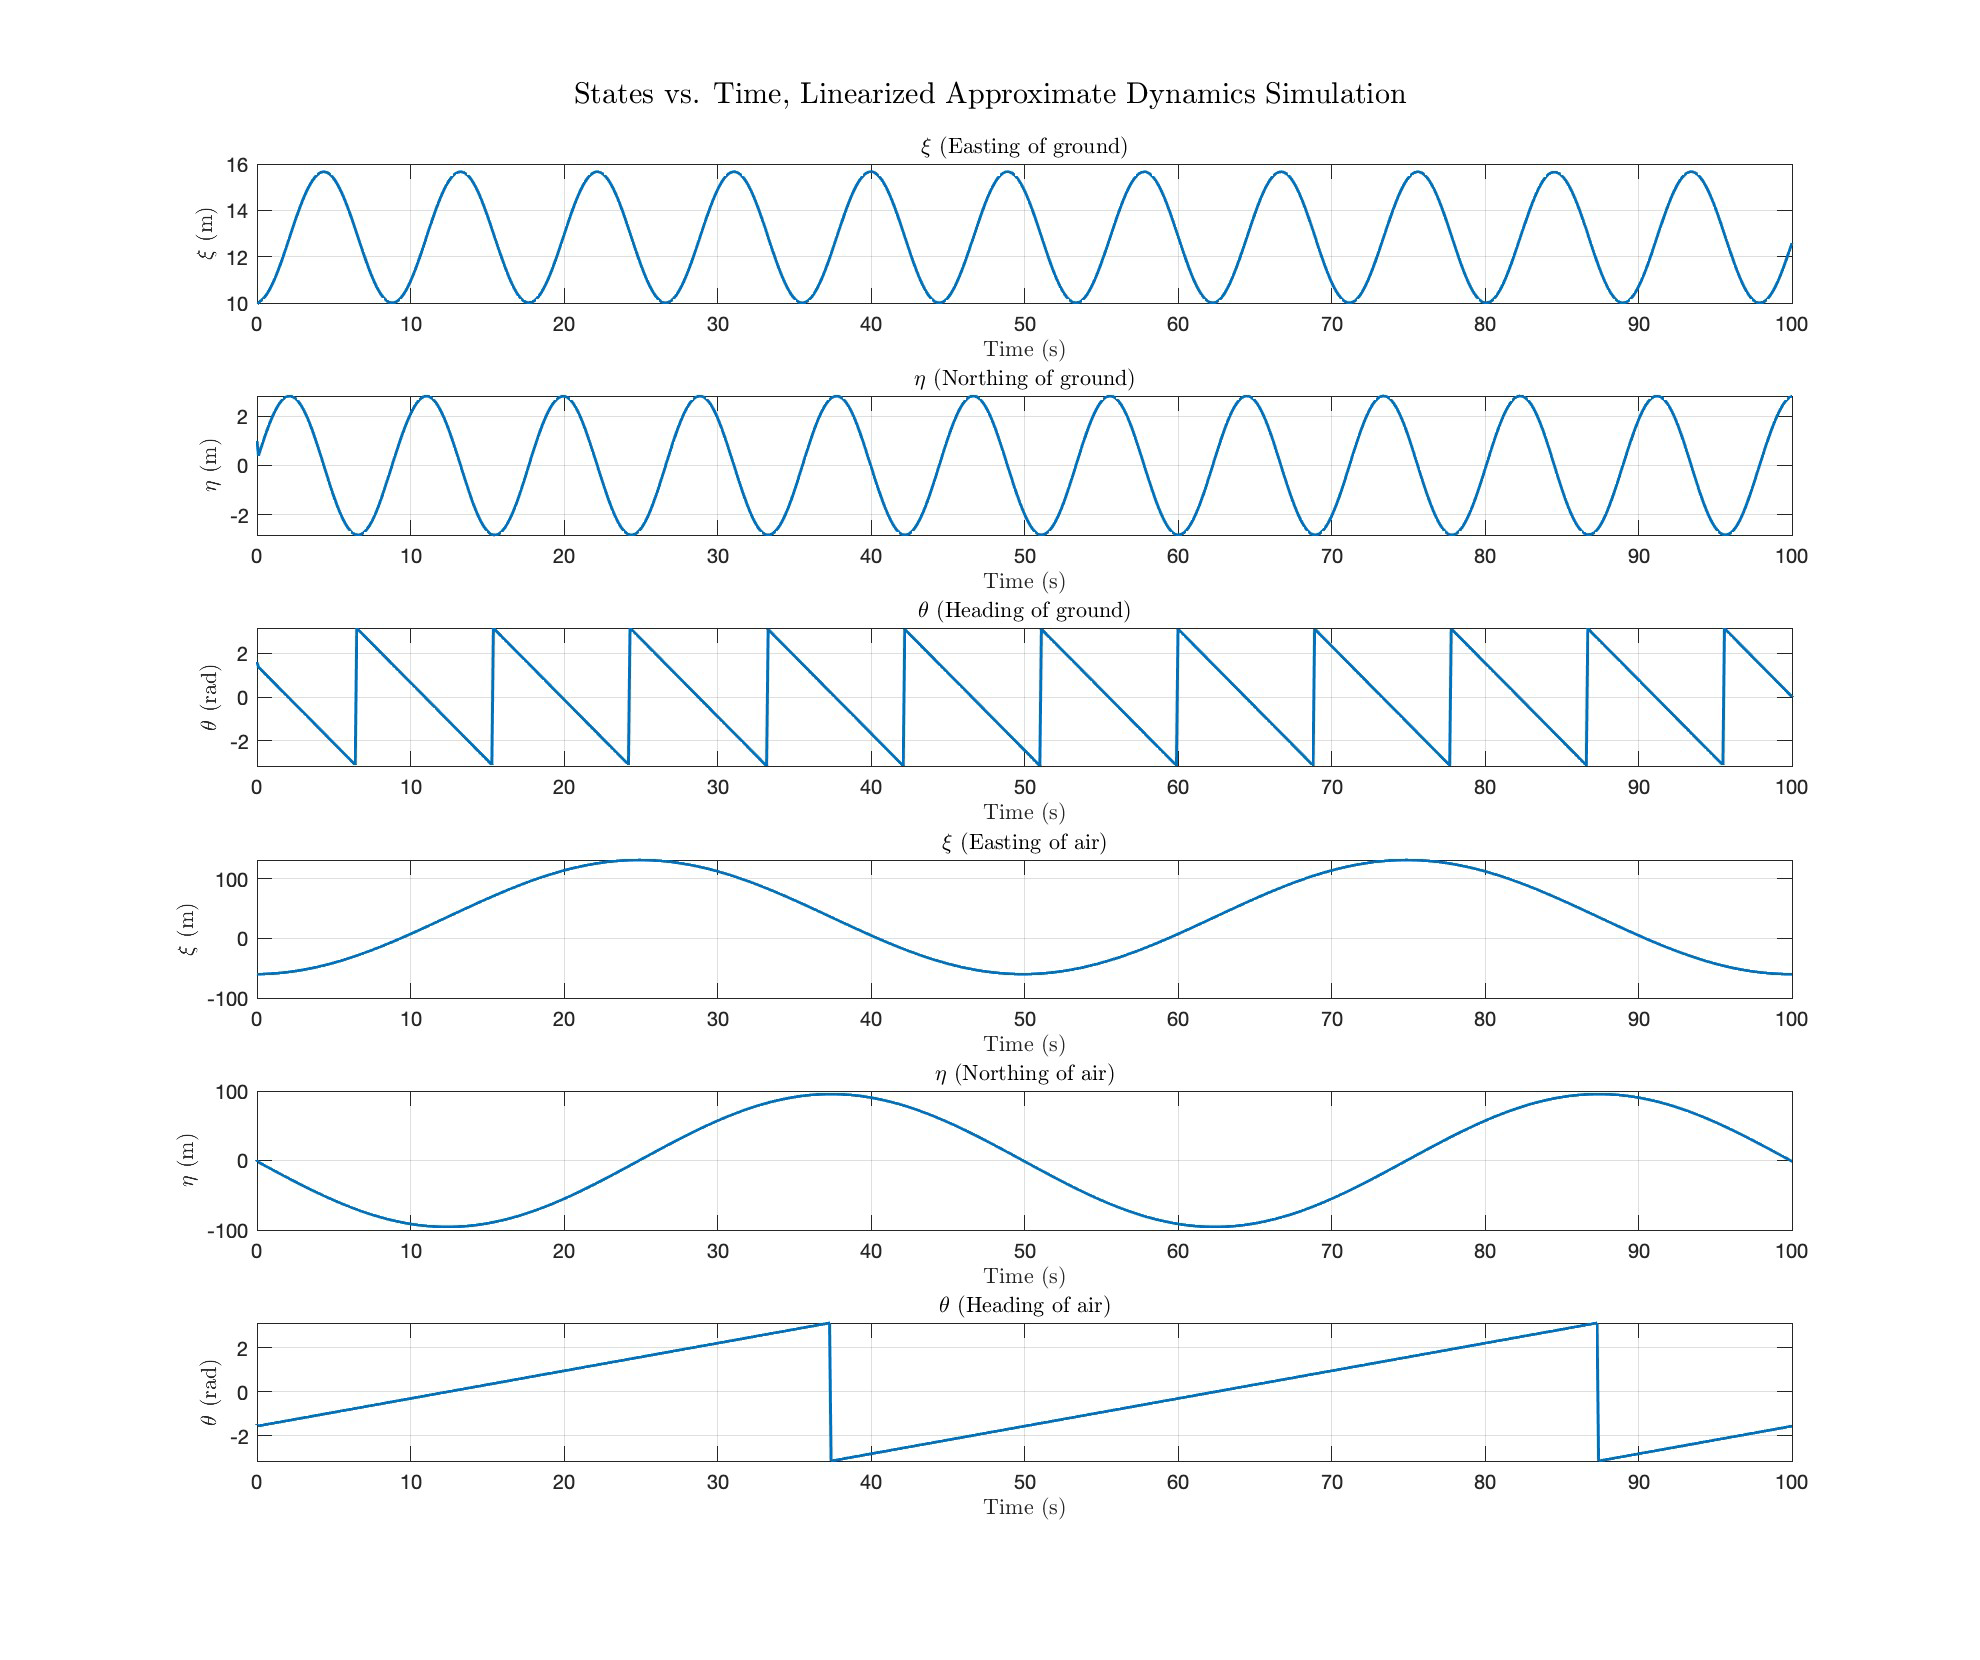
\includegraphics[scale=0.2]{LinearizedFullStateDynamics.png}
   \centering
   \captionof{figure}{Linearized Full State Dynamics}
\end{minipage}
 
 


The perturbation states from the same simulation are shown below.
\begin{minipage}[t]{1\linewidth}
   \vspace{-2ex}
   \centering
   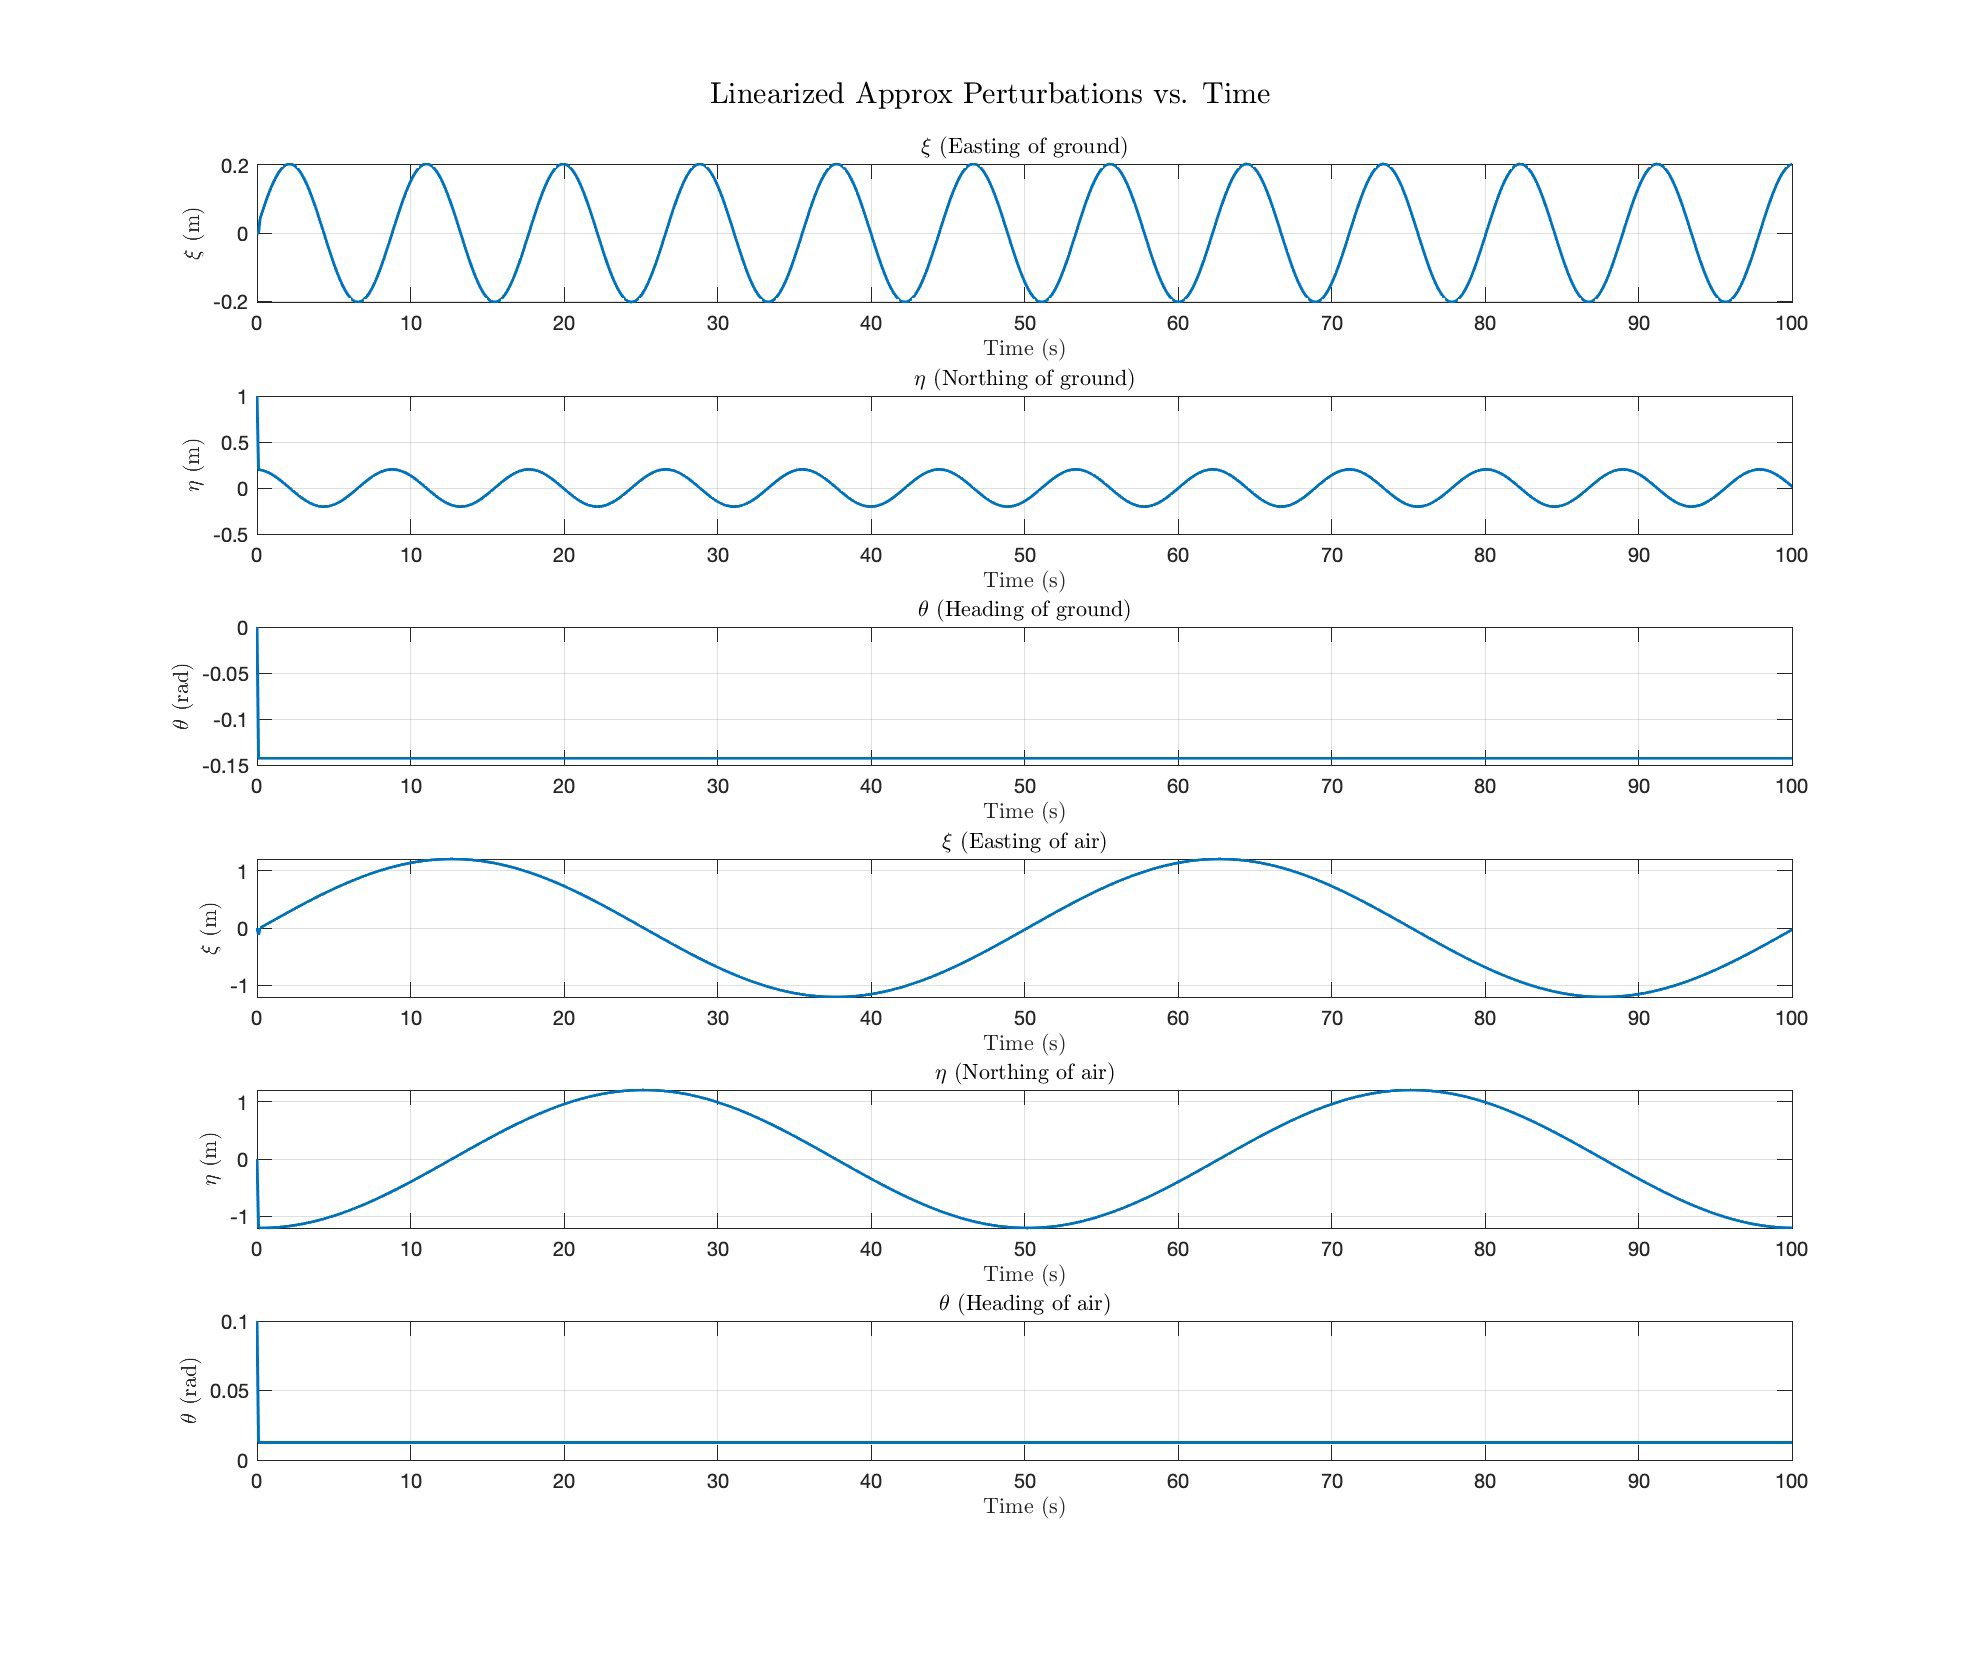
\includegraphics[scale=0.2]{LinearizedPerturbationStateDynamics.png}
   \captionof{figure}{Linearized Perturbation State Dynamics}
\end{minipage}

\newpage
\subsection{Part III} \\
To validate the DT LTV model we simulated in part 2, we performed a full nonlinear simulation of the system with the same initial perturbation state conditions of \(\delta x = [0, 1, 0, 0, 0, 0.1]\). We performed this simulation using ODE45 in MATLAB. The results of the simulation are shown below.

\begin{minipage}[t]{1\linewidth}
   \vspace{-2ex}
   \centering
   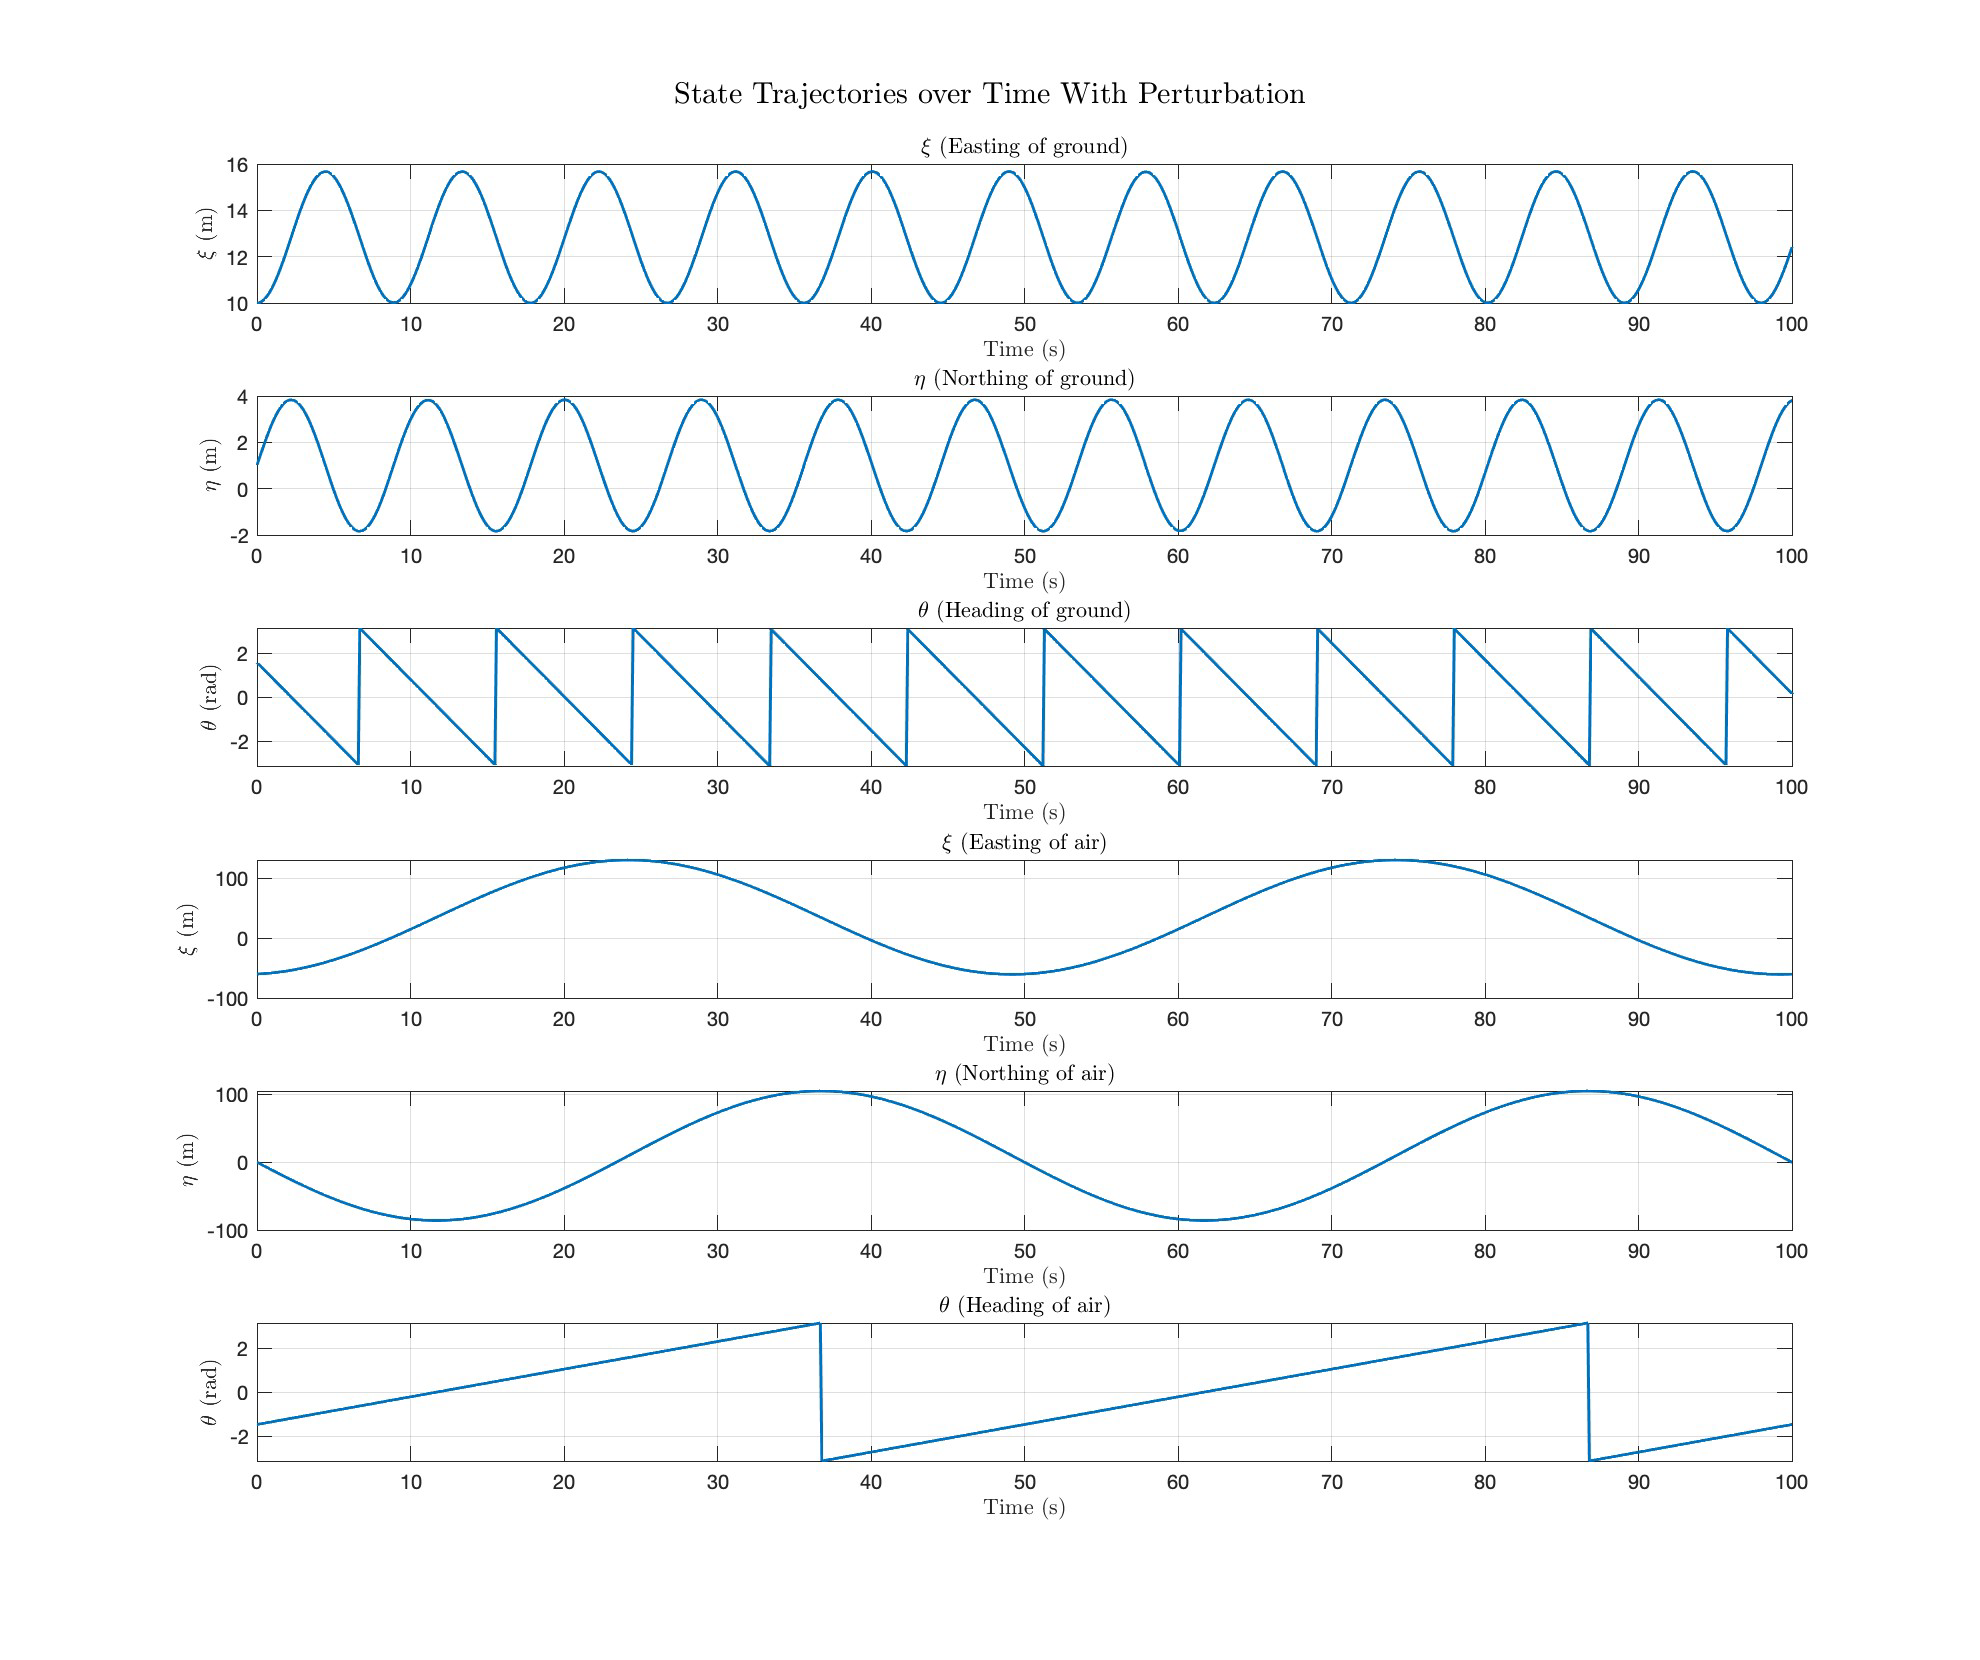
\includegraphics[scale=0.2]{NonlinearSimStateDynamics.png}
   \captionof{figure}{Non-linear Simulated State Dynamics}
\end{minipage}
\\~\\
\\~\\
The linearized approximate dynamics simulation results are very close to that of the nonlinear simulation. By closely comparing the two plots, we were able to observe a very slight phase shift between the states of the two simulations, but the linearized simulation matches the nonlinear simulation very well.
\end{framed}


\newpage

\section{Part II. STOCHASTIC NONLINEAR FILTERING}
\begin{framed}

\subsection{Part a.}

\subsection{Part b.}

\subsection{Part c.}



\end{framed}




\newpage
\section{Appendix}
\begin{framed}

We have attached a link to our team GitHub below. All code used to simulate the system and generate plots can be found at:
\\
\url{https://github.com/bernabei24/final_project_asen_5044_f24/tree/main}

\end{framed}


% \textbf{\\ Part II: Stochastic Nonlinear Filtering }
% \begin{framed}
   
% \end{framed}


\end{document}